The above equation can be expressed in the form 
\begin{align}
\vec{x}^T\vec{V}\vec{x}+2\vec{u}^T\vec{x}+f&=0 \label{eq:solutions/40/5/eq1}
\intertext{Comparing equation we get}
    \vec{V}=\vec{V}^T&=\myvec{6 & \frac{-5}{2}\\\frac{-5}{2} &-6}\label{eq:solutions/40/5/eqv}\\
    \vec{u}&=\myvec{7 \\ \frac{5}{2}}\label{eq:solutions/40/5/equ}\\
    f&=4\label{eq:solutions/40/5/eqfv}
\end{align}    
The above equation \eqref{eq:solutions/40/5/eq1} represents a pair of straight lines if
\begin{align}
    \begin{array}{|cc|}
\vec{V} & \vec{u}\\\vec{u}^T & f
\end{array}&=0\label{eq:solutions/40/5/eqcheck}
\end{align}
Verify the given equation as if it is pair of straight lines
\begin{align}
\Delta&=\begin{array}{|ccc|}
6 &\frac{-5}{2}& 7\\\frac{-5}{2} & -6 & \frac{5}{2}\\ 7 & \frac{5}{2} & 4
\end{array}\\
\implies \ 6\mydet{-6 & \frac{5}{2} \\ \frac{5}{2} & 4} 
		& -\frac{-5}{2}\mydet{-\frac{5}{2} & \frac{5}{2} \\ 7 & 4}
		+7\mydet{-\frac{5}{2} & -6 \\ 7 & \frac{5}{2}} = 0 \label{eq:solutions/40/5/eq10}\\
\implies \Delta&=0
\end{align}
Since equation \eqref{eq:solutions/40/5/eqcheck} is satisfied, we could say that the given equation represents two straight lines
\begin{align}
    \Delta_{V} &= \begin{array}{|cc|}
6 &\frac{-5}{2}\\\frac{-5}{2} & -6
\end{array}<0
\end{align}
Let the equations of lines be,
\begin{align}
	\brak{\vec{n_1}^T \vec{x} - c_1}\brak{\vec{n_1}^T \vec{x} - c_1} =
        \vec{x}^{T}\vec{Vx} + 2\vec{u}^{T}\vec{x} + f=0\label{eq:solutions/40/5/eq:eql03}
\end{align}
\begin{align}
\brak{\vec{n_1}^T\vec{x}-c_1}\brak{\vec{n_2}^T\vec{x}-c_2}
&=\vec{x}^T\myvec{6 & \frac{-5}{2} \\\frac{-5}{2} & -6}\vec{x}\notag\\
+2\myvec{7 & \frac{5}{2}}\vec{x}+4\label{eq:solutions/40/5/equate}\\
    \vec{n_1}*\vec{n_2} = \myvec{a\\2b\\c} &= \myvec{6\\-5\\-6}\label{eq:solutions/40/5/conv}\\
    c_2\vec{n_1}+c_1\vec{n_2}&=-2\myvec{7\\\frac{5}{2}}\label{eq:solutions/40/5/eqc1c2}\\
    c_1c_2&=4
\end{align}
The slopes of the lines are given by the roots of the polynomial 
\begin{align}
    &cm^2+2bm+a=0\label{eq:solutions/40/5/e}\\
    \implies m_i&=\frac{-b\pm{\sqrt{-\Delta_{V}}}}{c}\\
    \vec{n_i}&=k\myvec{-m_i\\1}
\end{align}
Substituting the given data in above equations \eqref{eq:solutions/40/5/e} we get,
\begin{align}
    &-6m^2-5m+6=0\\
    &\implies m_i=\frac{\frac{-5}{2}\pm{\sqrt{-(\frac{-169}{4})}}}{-6}\label{eq:solutions/40/5/m}
\intertext{Solving equation \eqref{eq:solutions/40/5/m} we get,}
    m_1&=-\frac{3}{2},  m_2=\frac{2}{3}\\
   % \vec{m_1}=\myvec{-2\\3}, \vec{m_2}=\myvec{3\\ 2}\\
   &= \vec{n_1}=\myvec{-3\\ -2}, \vec{n_2}=\myvec{-2\\3} \label{eq:solutions/40/5/eq:normal1}
\intertext{We know that,}
\vec{n_1}\ast \vec{n_2} = \myvec{a\\2b\\c} \label{eq:solutions/40/5/eq:conv1}
\end{align}
Verification using Toeplitz matrix, From equation \eqref{eq:solutions/40/5/eq:normal1}
\begin{align}
    \vec{n_1}=\myvec{-3&0\\-2&-3\\0&-2}
    \vec{n_2}=\myvec{-2\\3}\label{eq:solutions/40/5/eq:conv2}\\
\implies \myvec{-3&0\\-2&-3\\0&-2}\myvec{-2\\ 3} = \myvec{6\\-5\\-6} = \myvec{a\\2b\\c}\label{eq:solutions/40/5/eq:conv3}
\end{align}
$\implies$ Equation \eqref{eq:solutions/40/5/eq:normal1} satisfies \eqref{eq:solutions/40/5/eq:conv1}\\
$c_1$ and $c_2$ can be obtained as,
\begin{align}
\myvec{\vec{n_1} & \vec{n_2}}\myvec{c_2\\c_1}&=-2\vec{u} \label{eq:solutions/40/5/eq:aug1}
\end{align}
Substituting \eqref{eq:solutions/40/5/eq:normal1} in \eqref{eq:solutions/40/5/eq:aug1}, the augmented matrix is,
\begin{align}
\myvec{-3 & -2 & 14 \\ -2 & 3 & 5}
\xleftrightarrow[R_2\leftarrow R_2+2R_1]{R_1\leftarrow -R_1/3}
\myvec{1 &\frac{2}{3} &-\frac{14}{3} \\ 0& \frac{13}{3} & -\frac{13}{3}} \label{eq:solutions/40/5/eq:aug5}\\
\xleftrightarrow[R_1\leftarrow R_1-\frac{2}{3}R_2]{R_2\leftarrow \frac{3}{13}R_2}
\myvec{1 &0 &-4 \\ 0& 1 & -1} \label{eq:solutions/40/5/eq:aug2}\\
\implies c_1 = -4, c_2=-1 \label{eq:solutions/40/5/eq:const1}
\end{align}
Equations \eqref{eq:solutions/40/5/eq:eql03}, can be modified as,from \eqref{eq:solutions/40/5/eq:normal1} and \eqref{eq:solutions/40/5/eq:const1} in we get,
\begin{align}
    \myvec{-3 & -2}\vec{x}&=-4\\
    \myvec{-2 & 3}\vec{x}&=-1
\end{align}
\begin{multline}
\implies \brak{-3x-2y+4}\brak{-2x+3y+1}= 0\\
\implies \boxed{\brak{3x+2y-4}\brak{2x-3y-1} = 0} \label{eq:solutions/40/5/eq:line1}
\end{multline}
The angle between the lines can be expressed as, 
\begin{align}
	\vec{n_1}=\myvec{-3\\-2} , \quad \vec{n_2}=\myvec{-2\\3}\\
	\cos\theta=\frac{\vec{n_1}^T\vec{n_2}}{\norm{\vec{n_1}}\norm{\vec{n_2}}} \\
	\implies \quad \theta=\cos^{-1}({\frac{0}{\sqrt{169}}}) = 90\degree.
\end{align}
\begin{figure}[h]
    \centering
    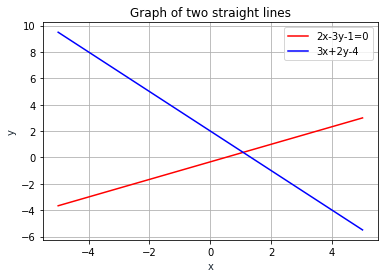
\includegraphics[width=\columnwidth]{./solutions/40/5/A6.png}
    \caption{Pair of straight lines}
    \label{eq:solutions/40/5/Fig :1}
\end{figure}
